% --------------- PROGETTAZIONE LOGICA ------------------------------------------

\newpage

\enlargethispage{1\linewidth}

\section{Progettazione Logica} 

\subsection{Stima del volume di dati}

\begin{tabular}{ | c  c  c | c  c  c | }
	\hline
	\rowcolor{airforceblue}
	\textbf{\color{white}Concetto} & \textbf{\color{white}Tipo} & \textbf{\color{white}Volume} & \textbf{\color{white}Concetto} & \textbf{\color{white}Tipo} & \textbf{\color{white}Volume}\\
	\hline
	\textsf{\small Passeggero} & \textsf{\small E} & \textsf{\small $ 200.000$} & \textsf{\small Aereo} & \textsf{\small E} & \textsf{\small $ 300 $}\\ %24.000
	\hline
	\textsf{\small Terminal} & \textsf{\small E} & \textsf{\small $ 3 $} & \textsf{\small Membro dell'equipaggio} & \textsf{\small E} & \textsf{\small $ 3.600 $}\\ %288.000
	\hline
	\textsf{\small Recarsi} & \textsf{\small R} & \textsf{\small $ 600.000 $} & \textsf{\small Far Parte} & \textsf{\small R} & \textsf{\small $ 300  $}\\ % recarsi prima 200.000 %24.000; far parte era 1.080.000
	\hline
	\textsf{\small Negozio} & \textsf{\small E} & \textsf{\small $ 50 $} & \textsf{\small Pista} & \textsf{\small E} & \textsf{\small $ 8 $}\\ % prima 7 piste
	\hline
	\textsf{\small Visitare} & \textsf{\small R} & \textsf{\small $ 10.000 $} & \textsf{\small Avviarsi} & \textsf{\small R} & \textsf{\small $ 2.400 $}\\ % visitare prima 50.000; prima avviarsi era 24.000
	\hline
	\textsf{\small Addetto di Scalo} & \textsf{\small E} & \textsf{\small $ 5.000 $} & \textsf{\small Via di rullaggio} & \textsf{\small E} & \textsf{\small $ 30 $}\\
	\hline
	\textsf{\small Interagire} & \textsf{\small R} & \textsf{\small $ 50.000 $} & \textsf{\small Ground Support Equipment} & \textsf{\small E} & \textsf{\small $ 300$}\\
	\hline
	\textsf{\small Addetto alla sicurezza} & \textsf{\small E} & \textsf{\small $ 500 $} & \textsf{\small Eseguire} & \textsf{\small R} & \textsf{\small $ 24.000 $}\\
	\hline
	\textsf{\small Controllare} & \textsf{\small R} & \textsf{\small $ 200.000 $} & \textsf{\small Tratta} & \textsf{\small E} & \textsf{\small $ 400 $}\\
	\hline
	\textsf{\small Aiutante per disabili} & \textsf{\small E} & \textsf{\small $ 50 $} & \textsf{\small Servizio} & \textsf{\small R} & \textsf{\small $ 4.000 $}\\
	\hline
	\textsf{\small Aiutare} & \textsf{\small R} & \textsf{\small $ 2.400 $} & \textsf{\small } & \textsf{\small } & \textsf{\small $ $}\\
	\hline
	\textsf{\small Volo} & \textsf{\small E} & \textsf{\small $ 4.000 $} & \textsf{\small Mantenimento} & \textsf{\small E} & \textsf{\small $ 200 $}\\ %volo era 24.000; prima era 1.000 volo
	\hline
	\textsf{\small Prendere} & \textsf{\small R} & \textsf{\small $ 4.000 $} & \textsf{\small Preservare} & \textsf{\small R} & \textsf{\small $ 6.000 $}\\ % prima era 12.000; prendere era 200.000.000
	\hline
	\textsf{\small Comporre} & \textsf{\small R} & \textsf{\small $ 1.200.000 $} & \textsf{\small Transitare} & \textsf{\small R} & \textsf{\small $ 9.000 $}\\ % prima 1.200.000; prima era 360.000.000
	\hline
	\textsf{\small Componente Aereo} & \textsf{\small E} & \textsf{\small $ 1.200.000 $} & \textsf{\small Assumere} & \textsf{\small R} & \textsf{\small $ 3.600 $}\\ % 1.200.000 prima; ora 1.200.000 * 300 aerei = 360.000.000
	\hline
	\textsf{\small } & \textsf{\small } & \textsf{\small $ $} & \textsf{\small } & \textsf{\small } & \textsf{\small $ $} \\
	\hline
	\textsf{\small Controllore} & \textsf{\small E} & \textsf{\small $ 30 $} & \textsf{\small Hangar} & \textsf{\small E} & \textsf{\small $ 30 $}\\
	\hline
	\textsf{\small Controllo} & \textsf{\small R} & \textsf{\small $ 5.000 $} & \textsf{\small Risiedere} & \textsf{\small R} & \textsf{\small $ 300 $}\\
	\hline
	\textsf{\small Torre di Controllo} & \textsf{\small E} & \textsf{\small $ 1 $} & \textsf{\small } & \textsf{\small } & \textsf{\small $ $}\\
	\hline
	\textsf{\small Radar} & \textsf{\small E} & \textsf{\small $ 5 $} & \textsf{\small } & \textsf{\small } & \textsf{\small $ $}\\
	\hline
	\textsf{\small Informare} & \textsf{\small R} & \textsf{\small $ 9.000 $} & \textsf{\small } & \textsf{\small } & \textsf{\small $ $}\\ % prima 6.000
	\hline
	\textsf{\small Comunicazione} & \textsf{\small R} & \textsf{\small $ 9.000 $} & \textsf{\small } & \textsf{\small } & \textsf{\small $ $}\\ % prima 6.000
	\hline
	\textsf{\small Rilevazione} & \textsf{\small R} & \textsf{\small $ 12.000 $} & \textsf{\small } & \textsf{\small } & \textsf{\small $ $}\\
	\hline
	\textsf{\small } & \textsf{\small } & \textsf{\small $ $} & \textsf{\small } & \textsf{\small } & \textsf{\small $ $}\\
	\hline
	\textsf{\small Compagnia Aerea} & \textsf{\small E} & \textsf{\small $ 30 $} & \textsf{\small } & \textsf{\small } & \textsf{\small $ $}\\
	\hline
	\textsf{\small Manutenzione} & \textsf{\small E} & \textsf{\small $ 50 $} & \textsf{\small } & \textsf{\small } & \textsf{\small $ $}\\
	\hline
	\textsf{\small } & \textsf{\small } & \textsf{\small $ $} & \textsf{\small } & \textsf{\small } & \textsf{\small $ $}\\
	\hline
	\textsf{\small Fornitori} & \textsf{\small E} & \textsf{\small $ 50 $} & \textsf{\small } & \textsf{\small } & \textsf{\small $ $}\\
	\hline
	\textsf{\small Rifornire} & \textsf{\small R} & \textsf{\small $ 5.000 $} & \textsf{\small } & \textsf{\small } & \textsf{\small $ $}\\
	\hline
	\textsf{\small Logistica} & \textsf{\small E} & \textsf{\small $ 50 $} & \textsf{\small } & \textsf{\small } & \textsf{\small $ $}\\
	\hline
	\textsf{\small Cargo} & \textsf{\small E} & \textsf{\small $ 50 $} & \textsf{\small } & \textsf{\small } & \textsf{\small $ $}\\
	\hline
	\textsf{\small Fornire} & \textsf{\small R} & \textsf{\small $ 5.000 $} & \textsf{\small } & \textsf{\small } & \textsf{\small $ $}\\
	\hline
	\textsf{\small Mantenere} & \textsf{\small R} & \textsf{\small $ 6.000 $} & \textsf{\small } & \textsf{\small } & \textsf{\small $ $}\\
	\hline
	\textsf{\small Caricare} & \textsf{\small R} & \textsf{\small $ 6.000 $} & \textsf{\small } & \textsf{\small } & \textsf{\small $ $}\\
	\hline
	\textsf{\small Possedere} & \textsf{\small R} & \textsf{\small $ 300 $} & \textsf{\small } & \textsf{\small } & \textsf{\small $ $}\\
	\hline
\end{tabular}

% ---- DESCRIZIONE DELLE OPERAZIONI PRINCIPALI E STIMA DELLA LORO FREQUENZA -----

\newpage

\subsection{Descrizione delle operazioni principale e stima della loro frequenza}

\textsf{\small Si fornisce, di seguito, una tabella riportante la descrizione e la relativa frequenza delle operazioni principali nell'Aeroporto.}\\

\begin{tabular}{ | c c c |} 
	\hline
	\rowcolor{airforceblue}
	\textbf{\color{white}Codice} & \textbf{\color{white}Operazione} & \textbf{\color{white}Frequenza} \\
	\hline
	\textsf{\small 01} & \textsf{\small Registrare un nuovo passeggero} & \textsf{\small $5000/\text{giorno}$} \\ % 200.000 / 30 = 6666.6 (-1000)
	\hline
	\textsf{\small 02} & \textsf{\small  Numero totale di componenti non funzionanti in un aereo.} & \textsf{\small $ 1/\text{mese} $} \\ 
	\hline
	\textsf{\small 03} & \textsf{\small Voli in partenza} & \textsf{\small $ 1000 / \text{mese} $} \\
	% Voli in partenza:
	% Ho preso la media del numero dei passeggeri che un aereo può portare
	% da questo sito (che mostra gli aerei più comuni) https://www.ponderweasel.com/how-many-people-can-fit-on-a-plane/?__cf_chl_managed_tk__=pmd_2mLayow7P2xTK3G5HcerVGqTNeA1cnsOiQfUmRb1Vok-1635365141-0-gqNtZGzNAxCjcnBszQh9
	% escludendo gli aerei privati e da singoli ed ho ottenuto:
	% una media pari a 
	% 525 + 220 + 189 + 290 + 451 + 366 + 172 / 7 = 316,14 -> 316
	% Se io ho scritto 5000 passeggeri / giorno, allora
	% 5000 / 316 = 15.82 -> 16 aerei per trasportare queste 5000 persone ogni giorno
	% in un mese 16 * 31 = 496 però tenendo conto che questa è una media così
	% e non tutti gli aerei possono portare tanto quanto il numero medio allora
	% metto 1000.
	\hline
	\textsf{\small 04} & \textsf{\small Voli in arrivo} & \textsf{\small $ 1000 / \text{mese} $} \\
	\hline
	\textsf{\small 05} & \textsf{\small Manutenzione di un aereo} & \textsf{\small $ 2000 / \text{mese} $} \\
	\hline
	\textsf{\small 06} & \textsf{\small Comunicazioni tra controllori e membri dell'equipaggio di un aereo} & \textsf{\small $ 1000 / \text{giorno} $} \\
	% [3 (departure) + 3 (arrival) + 3 + 3 + (eventuali emergenze) ] * (2000 / 30) = 800 / comunicazioni al giorno. oppure 15 * (2000 / 30) = 1000
	
	% oppure
	
	% 238 persone circa per aeroplano, 238 * 840 = 199.920 passeggeri
	% 840 voli / 30 giorni = 28 / voli al giorno
	
	% oppure
	
	% 130 passeggeri per volo.
	% 130 * 1540 = 200.200 passeggeri
	% 1540 voli / 30 giorni = 51 / voli giornalieri
	
	\hline
	\textsf{\small 07} & \textsf{\small Rifornimento di un aereo} & \textsf{\small $ 2000/ \text{mese} $} \\
	\hline
	\textsf{\small 08} & \textsf{\small Assunzione di nuovi addetti} & \textsf{\small $ 1000 / \text{anno}$} \\
	\hline
	\textsf{\small 09} & \textsf{\small Controllare numero di radar presenti all'aeroporto} & \textsf{\small $ 1 / \text{giorno}$} \\
	\hline
	\textsf{\small 10} & \textsf{\small Aerei nella Via di Rullaggio} & \textsf{\small $ 2000 / \text{mese}$} \\
	\hline
	\textsf{\small 11} & \textsf{\small Persone che comprano prodotti ai negozi} & \textsf{\small $ 1000 / \text{giorno} $} \\
	% Persone != Passeggeri e quindi le persone potrebbero essere di più dei passeggeri, però non tuti vanno per i negozi e ancora di meno sono quelli che comprano. Quindi quelli che visitano i negozi diciamo che sono 2000/giorno, ma quelli che comprano sono diciamo circa 1000/giorno o anche meno, magari 500.
	\hline
	\textsf{\small 12} & \textsf{\small Persone che si recano al Terminal} & \textsf{\small $ 5000 / \text{giorno} $} \\
	\hline
	\textsf{\small 13} & \textsf{\small Nuovi membri dell'equipaggio assunti da una compagnia} & \textsf{\small $ 500 / \text{anno}$} \\ % se gli addetti sono 1000 all'anno, questi saranno un po' di meno, immagino, diventare piloti richiede tempo.
	\hline
	\textsf{\small 14} & \textsf{\small Inserimento di aerei stazionati negli hangar} & \textsf{\small $ 500 / \text{mese} $} \\ % (Quite big) Boeing 747 : 5600 square feet, quite big hangar : 317000 square feet.
	% 317000 / 5600 = 56,6 -> 57
	% Gli hangar sono più di uno.
	\hline
	\textsf{\small 15} & \textsf{\small Calcolare l'età media dei passeggeri} & \textsf{\small $ 1 / \text{mese} $} \\
	\hline
	\textsf{\small 16} & \textsf{\small Ottenere il numero di aerei di una compagnia aerea.} & \textsf{\small $ 1 / \text{anno} $} \\
	\hline
	\textsf{\small 17} & \textsf{\small Numero di controllori in una Torre di Controllo} & \textsf{\small $ 1 / \text{anno} $} \\
	\hline
	\textsf{\small 18} & \textsf{\small Numero di macchinari presenti nell'Aeroporto} & \textsf{\small $ 1 / \text{mese} $} \\
	\hline
	\textsf{\small 19} & \textsf{\small Mostrare i controllori che erano in servizio dalle 08:00 alle 13:00} & \textsf{\small $ 1 / \text{mese} $} \\
	% L'aeroporto compra il carburante e poi lo vende alle compagnie aeree.
	% altre risorse possono essere di cibo, di acqua, di servizi di catering,ecc..
	\hline
	\textsf{\small 20} & \textsf{\small Numero aerei commerciali di una compagnia aerea} & \textsf{\small $ 1/ \text{mese} $} \\
	\hline
	\textsf{\small 21} & \textsf{\small Quantità di merci trasportate in media da un aereo commerciale} & \textsf{\small $ 1/ \text{mese} $} \\
	\hline
\end{tabular}

% ----- SCHEMI DI NAVIGAZIONE E TABELLE DEGLI ACCESSI --------------------------

\newpage

\enlargethispage{1\linewidth}

\subsection{Schemi di navigazione e tabelle degli accessi}

\textsf{\small Dopo aver stimato il volume dei dati ed elencato le principali operazioni, vengono riportati qui i loro relativi schemi di navigazione. \emph{Si considerino di doppio peso gli accessi in scrittura rispetto a quelli in lettura}.}\break

%\textsf{\small } & \textsf{\small } & \textsf{\small } &  \textsf{\small }\\
%\hline

% OP 1 | Registrare un nuovo passeggero

%\centering

\textbf{\small OP 1 | Registrare un nuovo passeggero}\\

\textsf{\small Un passeggero diventa tale quando compra un biglietto, altrimenti viene considerato semplicemente una persona.}\break

\begin{tabular}{ c c c c}
	%\textbf{\small OP 1 | Registrare un nuovo passeggero} & & & \\
	\hline
	\rowcolor{airforceblue}
	\textbf{\color{white}Concetto} & \textbf{\color{white}Costrutto} & \textbf{\color{white}Accesi} & \textbf{\color{white}Tipo}\\
	\hline
	\textsf{\small Passeggero} & \textsf{\small E} & \textsf{\small 1} &  \textsf{\small S}\\
	\hline
	\rowcolor{airforceblue}
	\textsf{\small } & \textsf{\small } & \textbf{\color{white}Totale: 1S $\rightarrow 10000$/giorno} \textsf{\small } & \textsf{\small }\\ % 2 * 5000/giorno = 10000/giorno
	\hline
\end{tabular}

\vspace{.6cm}

% OP 2 | Numero totale di componenti non funzionanti in un aereo.

\textbf{\small OP 2 | Numero totale di componenti non funzionanti in un aereo}\\
%\textsf{\small Tra le migliaia di persone giornaliere, non vengono necessariamente controllate tutte, ma solo quelle di cui si ha dei sospetti o si vogliono fare ulteriori accertamenti. (con controllo non intendo il check-in).}\break

\textsf{\small Ai fini della manutenzione degli aeromobili è necessario assicurarsi che tutte le componenti siano correttamente presenti e funzionanti.}\break

\begin{tabular}{ c c c c}
	%\textbf{\small OP 2 | Numero totale di componenti non funzionanti in un aereo.} & & & \\
	\hline
	\rowcolor{airforceblue}
	\textbf{\color{white}Concetto} & \textbf{\color{white}Costrutto} & \textbf{\color{white}Accesi} & \textbf{\color{white}Tipo}\\
	\hline
	\textsf{\small Componente Aereo} & \textsf{\small E} & \textsf{\small 1} &  \textsf{\small L}\\
	\hline
	\rowcolor{airforceblue}
	\textsf{\small } & \textsf{\small } & \textbf{\color{white}Totale: 1L$\rightarrow 1$/mese} \textsf{\small } & \textsf{\small }\\ 
	\hline
\end{tabular}

\vspace{.6cm}

% OP 3 | Voli in partenza

\textbf{\small OP 3 | Voli in partenza}\\

\begin{tabular}{ c c c c} 
	%\textbf{\small OP 3 | Voli in partenza} & & & \\
	\hline
	\rowcolor{airforceblue}
	\textbf{\color{white}Concetto} & \textbf{\color{white}Costrutto} & \textbf{\color{white}Accesi} & \textbf{\color{white}Tipo}\\
	\hline
	\textsf{\small Volo} & \textsf{\small E} & \textsf{\small 1} &  \textsf{\small L}\\
	\hline
	\textsf{\small Servizio} & \textsf{\small R} & \textsf{\small 1} &  \textsf{\small L}\\
	\hline
	\textsf{\small Tratta} & \textsf{\small E} & \textsf{\small 1} &  \textsf{\small L}\\
	\hline
	\rowcolor{airforceblue}
	\textsf{\small } & \textsf{\small } & \textbf{\color{white}Totale: 3L$\rightarrow 3000$/mese} \textsf{\small } & \textsf{\small }\\ %2000 * 3 / mese, anzi 1000 * 3 = 3000
	\hline
\end{tabular}

\vspace{.6cm}

% OP 4 | Voli in arrivo

\textbf{\small OP 4 | Voli in arrivo}\\

\begin{tabular}{ c c c c}
	%\textbf{\small OP 4 | Voli in arrivo} & & & \\
	\hline
	\rowcolor{airforceblue}
	\textbf{\color{white}Concetto} & \textbf{\color{white}Costrutto} & \textbf{\color{white}Accesi} & \textbf{\color{white}Tipo}\\
	\hline
	\textsf{\small Volo} & \textsf{\small E} & \textsf{\small 1} &  \textsf{\small L}\\
	\hline
	\textsf{\small Servizio} & \textsf{\small R} & \textsf{\small 1} &  \textsf{\small L}\\
	\hline
	\textsf{\small Tratta} & \textsf{\small E} & \textsf{\small 1} &  \textsf{\small L}\\
	\hline
	\rowcolor{airforceblue}
	\textsf{\small } & \textsf{\small } & \textbf{\color{white}Totale: 3L$\rightarrow 3000$/mese } \textsf{\small } & \textsf{\small }\\ % 2000 * 3 / mese = 6000 / mese
	\hline
\end{tabular}

\vspace{.6cm}

% OP 5 | Manutenzione di un aereo

\textbf{\small OP 5 | Manutenzione di un aereo}\\

\textsf{\small Il controllo periodico degli aerei è importante per la sicurezza di tutte le persone a bordo.}\break

\begin{tabular}{ c c c c} 
	%\textbf{\small OP 5 | Manutenzione di un aereo} & & & \\
	\hline
	\rowcolor{airforceblue}
	\textbf{\color{white}Concetto} & \textbf{\color{white}Costrutto} & \textbf{\color{white}Accesi} & \textbf{\color{white}Tipo}\\
	\hline
	\textsf{\small Mantenimento} & \textsf{\small E} & \textsf{\small 1} &  \textsf{\small L}\\
	\hline
	\textsf{\small Preservare} & \textsf{\small R} & \textsf{\small 30} &  \textsf{\small L}\\
	\hline
	\textsf{\small Aereo} & \textsf{\small E} & \textsf{\small 30} &  \textsf{\small L}\\
	\hline
	\rowcolor{airforceblue}
	\textsf{\small } & \textsf{\small } & \textbf{\color{white}Totale: 61L $\rightarrow 122.000$/mese} \textsf{\small } & \textsf{\small }\\ % 2000 * 3 = 6000 / mese
	\hline
\end{tabular}

\vspace{.6cm}

% OP 6 | Comunicazioni tra controllori e membri dell'equipaggio di un aereo

\pagebreak

\textbf{\small OP 6 | Comunicazioni tra controllori e membri dell'equipaggio di un aereo}\\

\textsf{\small La comunicazione tra torre di controllo, ovvero controllori e piloti è di vitale importanza per un volo regolare.}\break

\begin{tabular}{ c c c c}
	%\textbf{\small OP 6 | Comunicazioni tra controllori e membri dell'equipaggio di un aereo} & & & \\
	\hline
	\rowcolor{airforceblue}
	\textbf{\color{white}Concetto} & \textbf{\color{white}Costrutto} & \textbf{\color{white}Accesi} & \textbf{\color{white}Tipo}\\
	\hline
	\textsf{\small Torre di Controllo} & \textsf{\small E} & \textsf{\small 1} &  \textsf{\small L}\\
	\hline
	\rowcolor{airforceblue}
	\textsf{\small } & \textsf{\small } & \textbf{\color{white}Totale: 1L$\rightarrow 1000$/giorno } \textsf{\small } & \textsf{\small }\\ 
	\hline
\end{tabular}

\vspace{.6cm}

% OP 7 | Rifornimento di un aereo

%\newpage %\pagebreak

\textbf{\small OP 7 | Rifornimento di un aereo}\\

\textsf{\small Rifornire l'aereo di varie risorse di primaria importanza per il suo funzionamento, non soltanto del carburante, ma anche di cibo, acqua, servizi di catering,ecc.. per il normale svolgimento delle operazioni e per il soddisfacimento dei bisogni dei passeggeri.}\break

\begin{tabular}{ c c c c}
	%\textbf{\small OP 7 | } & & & \\
	\hline
	\rowcolor{airforceblue}
	\textbf{\color{white}Concetto} & \textbf{\color{white}Costrutto} & \textbf{\color{white}Accesi} & \textbf{\color{white}Tipo}\\
	\hline
	\textsf{\small Logistica} & \textsf{\small E} & \textsf{\small 1} &  \textsf{\small L}\\
	\hline
	\textsf{\small Fornire} & \textsf{\small R} & \textsf{\small 100} &  \textsf{\small L}\\
	\hline
	\textsf{\small Cargo} & \textsf{\small E} & \textsf{\small 100} &  \textsf{\small L}\\
	\hline
	\rowcolor{airforceblue}
	\textsf{\small } & \textsf{\small } & \textbf{\color{white}Totale: 201L$\rightarrow 402.000$/mese } \textsf{\small } & \textsf{\small }\\ % 2000 * 3 = 6000/mese
	\hline
\end{tabular}

\vspace{.6cm}

% OP 8 | Assunzione di nuovi addetti

\textbf{\small OP 8 | Assunzione di nuovi addetti}\\

\begin{tabular}{ c c c c}
	%\textbf{\small OP 8 | } & & & \\
	\hline
	\rowcolor{airforceblue}
	\textbf{\color{white}Concetto} & \textbf{\color{white}Costrutto} & \textbf{\color{white}Accesi} & \textbf{\color{white}Tipo}\\
	\hline
	\textsf{\small Addetto di Scalo} & \textsf{\small E} & \textsf{\small 1} &  \textsf{\small S}\\
	\hline
	\rowcolor{airforceblue}
	\textsf{\small } & \textsf{\small } & \textbf{\color{white}Totale: 1S$\rightarrow 2000$/anno } \textsf{\small } & \textsf{\small }\\ % 2 * 1000 = 2000
	\hline
\end{tabular}

\vspace{.6cm}

% OP 9 | Controllare numero di radar presenti all'aeroporto

\textbf{\small OP 9 | Controllare numero di radar presenti all'aeroporto }\\

\textsf{\small Allo scopo di mantenere sicure le operazioni aeroportuali è necessario un controllo periodico dei radar presenti nell'aeroporto.}\break

\begin{tabular}{ c c c c} 
	%\textbf{\small OP 9 | } & & & \\
	\hline
	\rowcolor{airforceblue}
	\textbf{\color{white}Concetto} & \textbf{\color{white}Costrutto} & \textbf{\color{white}Accesi} & \textbf{\color{white}Tipo}\\
	\hline
	\textsf{\small Radar} & \textsf{\small E} & \textsf{\small 1} &  \textsf{\small L}\\
	\hline
	\rowcolor{airforceblue}
	\textsf{\small } & \textsf{\small } & \textbf{\color{white}Totale: 1L$\rightarrow 1$/giorno } \textsf{\small } & \textsf{\small }\\
	\hline
\end{tabular}

\vspace{.6cm}

% OP 10 | Aerei nella Via di Rullaggio

\textbf{\small OP 10 | Aerei nella Via di Rullaggio}\\

\begin{tabular}{ c c c c} 
	%\textbf{\small OP 10 | } & & & \\
	\hline
	\rowcolor{airforceblue}
	\textbf{\color{white}Concetto} & \textbf{\color{white}Costrutto} & \textbf{\color{white}Accesi} & \textbf{\color{white}Tipo}\\
	\hline
	\textsf{\small Via di Rullaggio} & \textsf{\small E} & \textsf{\small 30} &  \textsf{\small L}\\
	\hline
	\rowcolor{airforceblue}
	\textsf{\small } & \textsf{\small } & \textbf{\color{white}Totale: 30L$\rightarrow 60.000$/mese } \textsf{\small } & \textsf{\small }\\
	\hline
\end{tabular}

\vspace{.6cm}

\pagebreak

% OP 11 | Acquirenti ai negozi

\textbf{\small OP 11 | Acquirenti ai negozi}\\

\begin{tabular}{ c c c c}
	%\textbf{\small OP 11 | } & & & \\
	\hline
	\rowcolor{airforceblue}
	\textbf{\color{white}Concetto} & \textbf{\color{white}Costrutto} & \textbf{\color{white}Accesi} & \textbf{\color{white}Tipo}\\
	\hline
	\textsf{\small Persona} & \textsf{\small E} & \textsf{\small 1} &  \textsf{\small L}\\
	\hline
	\textsf{\small Visitare} & \textsf{\small R} & \textsf{\small 50} &  \textsf{\small L}\\
	\hline
	\textsf{\small Negozio} & \textsf{\small E} & \textsf{\small 50} &  \textsf{\small L}\\
	\hline
	\rowcolor{airforceblue}
	\textsf{\small } & \textsf{\small } & \textbf{\color{white}Totale: 101L$\rightarrow 101.000$/giorno } \textsf{\small } & \textsf{\small }\\ % 1000 * 3 = 3000
	\hline
\end{tabular}

\vspace{.6cm}

% OP 12 | Passeggeri che si recano al Terminal

\textbf{\small OP 12 | Persone che si recano al Terminal}\\

\begin{tabular}{ c c c c}
	%\textbf{\small OP 12 | } & & & \\
	\hline
	\rowcolor{airforceblue}
	\textbf{\color{white}Concetto} & \textbf{\color{white}Costrutto} & \textbf{\color{white}Accesi} & \textbf{\color{white}Tipo}\\
	\hline
	\textsf{\small Passeggero} & \textsf{\small E} & \textsf{\small 1} &  \textsf{\small L}\\
	\hline
	\textsf{\small Recarsi} & \textsf{\small R} & \textsf{\small 3} &  \textsf{\small L}\\
	\hline
	\textsf{\small Terminal} & \textsf{\small E} & \textsf{\small 3} &  \textsf{\small L}\\
	\hline
	\hline
	\rowcolor{airforceblue}
	\textsf{\small } & \textsf{\small } & \textbf{\color{white}Totale: 7L$\rightarrow 35.000$/giorno } \textsf{\small } & \textsf{\small }\\ % 2 * 5000 = 10000, 5000 * 3 = 15000/giorno
	\hline
\end{tabular}

\vspace{.6cm}

% OP 13 | Nuovi membri dell'equipaggio assunti da una compagnia

\textbf{\small OP 13 | Nuovi membri dell'equipaggio assunti da una compagnia}\\

\begin{tabular}{ c c c c} 
	%\textbf{\small OP 13 | } & & & \\
	\hline
	\rowcolor{airforceblue}
	\textbf{\color{white}Concetto} & \textbf{\color{white}Costrutto} & \textbf{\color{white}Accesi} & \textbf{\color{white}Tipo}\\
	\hline
	\textsf{\small Membro dell'Equipaggio} & \textsf{\small E} & \textsf{\small 1} &  \textsf{\small S}\\
	\hline
	\textsf{\small Assumere} & \textsf{\small R} & \textsf{\small 1} &  \textsf{\small S}\\
	\hline
	\textsf{\small Compagnia Aerea} & \textsf{\small E} & \textsf{\small 1} &  \textsf{\small S}\\
	\hline
	\rowcolor{airforceblue}
	\textsf{\small } & \textsf{\small } & \textbf{\color{white}Totale: 3S$\rightarrow 3000$/anno } \textsf{\small } & \textsf{\small }\\ % 2 * 500 = 1000
	\hline
\end{tabular}

\vspace{.6cm}

% OP 14  | Inserimento di aerei stazionati negli Hangar

\textbf{\small OP 14 | Inserimento di aerei stazionati negli Hangar}\\

\begin{tabular}{ c c c c}
	%\textbf{\small OP 14 | } & & & \\
	\hline
	\rowcolor{airforceblue}
	\textbf{\color{white}Concetto} & \textbf{\color{white}Costrutto} & \textbf{\color{white}Accesi} & \textbf{\color{white}Tipo}\\
	\hline
	\textsf{\small Aereo} & \textsf{\small E} & \textsf{\small 10} &  \textsf{\small S}\\
	\hline
	\rowcolor{airforceblue}
	\textsf{\small } & \textsf{\small } & \textbf{\color{white}Totale: 20S$\rightarrow 10.000$/mese } \textsf{\small } & \textsf{\small }\\ % 2 * 500 == 1000
	\hline
\end{tabular}

\vspace{.6cm}

% OP 15 | Calcolare l'età media dei passeggeri

\textbf{\small OP 15 | Calcolare l'età media dei passeggeri}\\

%\flushleft

\textsf{\small Ai fini statistici, per capire quali persone viaggiano di più, a che età e dove, ecc.. Viene registrata e calcolata l'età media delle persone e vari altri dati.}\break

%\centering

\begin{tabular}{ c c c c}
	%\textbf{\small OP 15 | } & & & \\
	\hline
	\rowcolor{airforceblue}
	\textbf{\color{white}Concetto} & \textbf{\color{white}Costrutto} & \textbf{\color{white}Accesi} & \textbf{\color{white}Tipo}\\
	\hline
	\textsf{\small Passeggero} & \textsf{\small E} & \textsf{\small 1} &  \textsf{\small L}\\
	\hline
	\rowcolor{airforceblue}
	\textsf{\small } & \textsf{\small } & \textbf{\color{white}Totale: 1L$\rightarrow 1$/mese } \textsf{\small } & \textsf{\small }\\
	\hline
\end{tabular}

\vspace{.6cm}

% OP 16  | Ottenere il numero di aerei di una compagnia aerea

\textbf{\small OP 16 | Ottenere il numero di aerei di una compagnia aerea}\\

\begin{tabular}{ c c c c}
	%\textbf{\small OP 16 | } & & & \\
	\hline
	\rowcolor{airforceblue}
	\textbf{\color{white}Concetto} & \textbf{\color{white}Costrutto} & \textbf{\color{white}Accesi} & \textbf{\color{white}Tipo}\\
	\hline
	\textsf{\small Compagnia Aerea} & \textsf{\small E} & \textsf{\small 1} &  \textsf{\small L}\\
	\hline
	\rowcolor{airforceblue}
	\textsf{\small } & \textsf{\small } & \textbf{\color{white}Totale: 1l$\rightarrow 1$/anno } \textsf{\small } & \textsf{\small }\\
	\hline
\end{tabular}

\vspace{.6cm}

\pagebreak

% OP 17  | Numero di controllori in una Torre di Controllo

\textbf{\small OP 17 | Numero di controllori in una Torre di Controllo}\\

\begin{tabular}{ c c c c}
	%\textbf{\small OP 17 | } & & & \\
	\hline
	\rowcolor{airforceblue}
	\textbf{\color{white}Concetto} & \textbf{\color{white}Costrutto} & \textbf{\color{white}Accesi} & \textbf{\color{white}Tipo}\\
	\hline
	\textsf{\small Torre di Controllo} & \textsf{\small E} & \textsf{\small 1} &  \textsf{\small L}\\
	\hline
	\rowcolor{airforceblue}
	\textsf{\small } & \textsf{\small } & \textbf{\color{white}Totale: 1L$\rightarrow 1$/anno } \textsf{\small } & \textsf{\small }\\
	\hline
\end{tabular}

\vspace{.6cm}

% OP 18  | Numero di macchinari presenti nell'Aeroporto

\textbf{\small OP 18 | Numero di macchinari presenti nell'Aeroporto}\\

\textsf{\small Per il controllo,la manutenzione dei vari macchinari e per la corretta esecuzione delle normali attività aeroportuali.}\break

\begin{tabular}{ c c c c}
	%\textbf{\small OP 18 | } & & & \\
	\hline
	\rowcolor{airforceblue}
	\textbf{\color{white}Concetto} & \textbf{\color{white}Costrutto} & \textbf{\color{white}Accesi} & \textbf{\color{white}Tipo}\\
	\hline
	\textsf{\small Ground Support Equipment } & \textsf{\small E} & \textsf{\small 1} &  \textsf{\small L}\\
	\hline
	\rowcolor{airforceblue}
	\textsf{\small } & \textsf{\small } & \textbf{\color{white}Totale: 1L$\rightarrow 1$/mese } \textsf{\small } & \textsf{\small }\\
	\hline
\end{tabular}

\vspace{.6cm}

% OP 19  | Approvvigionamento dell'aereo

\textbf{\small OP 19 | Mostrare i controllori che erano in servizio dalle 08:00 alle 13:00}\\

\begin{tabular}{ c c c c}
	%\textbf{\small OP 19 | } & & & \\
	\hline
	\rowcolor{airforceblue}
	\textbf{\color{white}Concetto} & \textbf{\color{white}Costrutto} & \textbf{\color{white}Accesi} & \textbf{\color{white}Tipo}\\
	\hline
	\textsf{\small Controllore} & \textsf{\small E} & \textsf{\small 1} &  \textsf{\small L}\\
	\hline
	\textsf{\small Operare} & \textsf{\small R} & \textsf{\small 1} &  \textsf{\small L}\\
	\hline
	\textsf{\small Torre di Controllo} & \textsf{\small E} & \textsf{\small 1} &  \textsf{\small L}\\
	\hline
	\rowcolor{airforceblue}
	\textsf{\small } & \textsf{\small } & \textbf{\color{white}Totale: 3L$\rightarrow 3$/ mese} \textsf{\small } & \textsf{\small }\\
	\hline
\end{tabular}

\vspace{.6cm}

% OP 20  | Numero aerei commerciali di una compagnia aerea

\textbf{\small OP 20 | Numero aerei commerciali di una compagnia aerea}\\

\begin{tabular}{ c c c c}
	%\textbf{\small OP 20 | } & & & \\
	\hline
	\rowcolor{airforceblue}
	\textbf{\color{white}Concetto} & \textbf{\color{white}Costrutto} & \textbf{\color{white}Accesi} & \textbf{\color{white}Tipo}\\
	\hline
	\textsf{\small Aereo} & \textsf{\small E} & \textsf{\small 1} &  \textsf{\small L}\\
	\hline
	\rowcolor{airforceblue}
	\textsf{\small } & \textsf{\small } & \textbf{\color{white}Totale: 1L$\rightarrow 1$/mese } \textsf{\small } & \textsf{\small }\\
	\hline
\end{tabular}

\vspace{.6cm}

% OP 21  | Quantità di merci trasportate in media da un aereo commerciale

\textbf{\small OP 21 | Quantità di merci trasportate in media da un aereo commerciale}\\

\textsf{\small Per tenere traccia di quante merci sono state vendute e trasportate da una compagnia aerea.}\break

\begin{tabular}{ c c c c}
	%\textbf{\small OP 21 | } & & & \\
	\hline
	\rowcolor{airforceblue}
	\textbf{\color{white}Concetto} & \textbf{\color{white}Costrutto} & \textbf{\color{white}Accesi} & \textbf{\color{white}Tipo}\\
	\hline
	\textsf{\small Aereo} & \textsf{\small E} & \textsf{\small 1} &  \textsf{\small L}\\
	\hline
	\rowcolor{airforceblue}
	\textsf{\small } & \textsf{\small } & \textbf{\color{white}Totale: 1L$\rightarrow 1$/mese } \textsf{\small } & \textsf{\small }\\
	\hline
\end{tabular}

%\flushleft

% --------------- RAFFINAMENTO DELLO SCHEMA ------------------------------------

\newpage

\subsection{Raffinamento dello schema}

%\subsubsection{Eliminazione gerarchie}
\textbf{Eliminazione delle gerarchie}\\
\textsf{\small Per quanto riguarda l'eliminazione delle gerarchie, ho deciso di adottare il collasso verso l'alto, come soluzione del problema.}\break 

% Collasso verso l'alto: Accorpare le entità figlie nel genitore

% Collasso verso il basso: Accorpare il genitore nelle entità figlie

\textsf{\small Ho individuato 9 gerarchie che ho collassato verso l'alto e aggiunto loro gli attributi \emph{Tipologia} o \emph{Ruolo}, ovvero \emph{Componente dell'aereo}, \emph{Membro dell'equipaggio}, \emph{Radar}, \emph{Controllore}, \emph{Addetto di scalo}, \emph{Negozio}, \emph{Ground Support Equipment},\emph{Tratta}, \emph{Persone}.}\\

\textbf{Eliminazione degli attributi compositi}

\textsf{\small Non è stato fatto uso di attributi compositi perciò non è stato necessario assestare in alcun modo.}\break %assestato, situazione/contesto.

\textbf{Scelte delle chiavi primarie}

\textsf{\small Nello schema proposto sono già presenti le chiavi primarie per tutte le entità, identificate ciascuna da un proprio codice univoco.}\break

\textbf{Eliminazione degli identificatori esterni}

\textsf{\small A seguito delle analisi compiute è stato determinato di rimuovere le seguenti relazioni:}\\ %deciso


\begin{itemize} 
	%\item \textsf{\small Relazione \emph{appartenere} tra \textbf{PASSEGGERO} e \textbf{BAGAGLIO}, importando \emph{Num. Bagagli} in \textbf{PASSEGGERO}.} %TODO: attributo numero valigie al posto delle relazione PASSEGGERO e BAGAGLIO (o VALIGIA)
	%\item \textsf{\small Relazione \emph{appartenere} tra \textbf{Passeggero} e \textbf{Bagaglio}, importando \emph{CodBagaglio} in \textbf{Persona}.}
	%\item \textsf{\small Associazione \emph{disporre} tra \textbf{AEREO} e \textbf{COMPAGNIA AEREA}, introducendo \emph{Num. Aerei} in \textbf{COMPAGNIA AEREA}.} %TODO: forse questa l'ho già cancellata nello schema?!
	%\item \textsf{\small } %TODO: Tra AEREO e COMPONENTE DELL'AEREO potrei mettere un attributo Num. Componenti
	%\item \textsf{\small \emph{Operare} tra \textbf{CONTROLLORE} e \textbf{TORRE DI CONTROLLO}, usando invece un attributo \emph{Num. Controllori} in \textbf{TORRE DI CONTROLLO}.} %TODO: questo attributo Num. Controllori ce l'ho già.
	%\item \textsf{\small \emph{Risiedere} tra \textbf{AEREO} ed \textbf{HANGAR} , usufruendo di un attributo \emph{Hangar[0:1]} in \textbf{AEREO} per sapere se l'aereo si trova nell'hangar e anche in quale.} %TODO: Al posto della relazione RISIEDERE tra AEREO ed HANGAR, magari potrei mettere direttamente un attributo in AEREO per sapere dove risiede e se sta risiedendo lì. tipo [0:1]
	
	%\item \textsf{\small \emph{Far parte} tra \textbf{AEREO} e \textbf{MEMBRO DELL'EQUIPAGGIO}, potrei avvalermi di un attributo \emph{Num. Equipaggio} nell'entià \textbf{AEREO}.} %TODO: AEREO e MEMBRO DELL'EQUIPAGGIO, piuttosto potrei avere un attributo Num.Equipaggio (che in realtà già ho). 
	%\item \textsf{\small \emph{Assumere} tra \textbf{COMPAGNIA AEREA} e \textbf{MEMBRO DELL'EQUIPAGGIO}, utilizzando un attributo \emph{Num. Dipendenti} o \emph{Num. Personale}.}%TODO: In realtà, ho già questo attributo in COMPAGNIA AEREA.
	
	%\item \textsf{\small }%TODO: relazioni OPERATA ed ESEGUITA in una GERARCHIA di MANUTENZIONE, (mah insomma)
	\item \textsf{\small \emph{Servire} tra \textbf{Persona} e \textbf{Servizio Clienti} importando \emph{CodServizio} in \textbf{Persona}.}
	\item \textsf{\small \emph{Visitare} tra \textbf{Persona} e \textbf{Negozio} importando \emph{CodNegozio} in \textbf{Persona}.}
	\item \textsf{\small \emph{Recarsi} tra \textbf{Terminal} e \textbf{Persona}, importando \emph{CodTerminal} in \textbf{Persona}.}
	\item \textsf{\small \emph{Intervenire} tra \textbf{Centro di Controllo d'Aerea} e \textbf{Persona}, importando \emph{CodCentro} in \textbf{Persona}.}
	\item \textsf{\small \emph{Informare} tra \textbf{Persona} e \textbf{Radar}, importando \emph{CodRadar} in \textbf{Persona}.}
	\item \textsf{\small \emph{Contattare} tra \textbf{Persona} e \textbf{Soccorsi}, trasferendo \emph{CodSoccorso} in \textbf{Persona}.}
	\item \textsf{\small \emph{Appartenere} tra \textbf{Persona} e \textbf{Bagaglio}, trasportando \emph{CodiceFiscale} in \textbf{Bagaglio}.}
	\item \textsf{\small \emph{Accertare} tra \textbf{Persona} e \textbf{Bagaglio}, importando \emph{CodiceFiscale} in \textbf{Bagaglio}.}
	\item \textsf{\small \emph{Adempiere} tra \textbf{Persona} e \textbf{Mantenimento}, importando \emph{CodMantenimento} in \textbf{Persona}. }
	\item \textsf{\small \emph{Rifornire} tra \textbf{Persona} e \textbf{Logistica}, trasferendo \emph{CodLogistica} in \textbf{Persona}. }
	\item \textsf{\small \emph{Prendere} tra \textbf{Volo} e \textbf{Persona}, inserendo \emph{CodVolo} in \textbf{Persona}.}
	\item \textsf{\small \emph{Comunicazione} tra \textbf{Torre di Controllo} e \textbf{Persona}, aggiungendo \emph{CodTorre} in \textbf{Persona}.}
	\item \textsf{\small \emph{Possedere} tra \textbf{Compagnia Aerea} e \textbf{Negozio}, importando \emph{CodCompagnia} in \textbf{Negozio}.}
	\item \textsf{\small \emph{Costituire} tra \textbf{Gate} e \textbf{Terminal}, trasferendo \emph{CodTerminal} in \textbf{Gate}.}
	\item \textsf{\small \emph{Rilevazione} tra \textbf{Radar} e \textbf{Aereo}, inserendo \emph{CodAereo} in \textbf{Radar}.}
	\item \textsf{\small \emph{Eseguire} tra \textbf{Ground Support Equipment} e \textbf{Mantenimento}, immettendo \emph{CodMacchinario} in \textbf{Mantenimento}.}
	\item \textsf{\small \emph{Detenere} tra \textbf{Aereo} e \textbf{Volo}, incorporando \emph{CodAereo} in \textbf{Volo}.}
	\item \textsf{\small \emph{Servizio} tra \textbf{Tratta} e \textbf{Volo}, allegando \emph{CodTratta} in \textbf{Volo}.}
	\item \textsf{\small \emph{Preservare} tra \textbf{Aereo} e \textbf{Mantenimento}, conglobando \emph{CodAereo} in \textbf{Mantenimento}.}
	\item \textsf{\small \emph{Transitare} tra \textbf{Aereo} e \textbf{Via di Rullaggio}, accorpando \emph{CodVia} in \textbf{Aereo}.}
	\item \textsf{\small \emph{Avviarsi} tra \textbf{Aereo} e \textbf{Pista},inglobando \emph{CodPista} in \textbf{Aereo}.}
	\item \textsf{\small \emph{Comporre} tra \textbf{Aereo} e \textbf{Componente dell'aereo}, inserendo \emph{CodAereo} in \textbf{Componente dell'aereo}.} % prima era l'incontrario. ma non si può per via delle cardinalità
	\item \textsf{\small \emph{Caricare} tra \textbf{Cargo} ed \textbf{Aereo},importando \emph{CodAereo} in \textbf{Cargo}.}
	\item \textsf{\small \emph{Mantenere} tra \textbf{Persona} e \textbf{Aereo}, aggiungendo \emph{CodAereo} in \textbf{Persona}.}
	\item \textsf{\small \emph{Risiedere} tra \textbf{Aereo} ed \textbf{Hangar}, trasferendo \emph{CodHangar} in \textbf{Aereo}.}
	\item \textsf{\small \emph{Tutelare} tra \textbf{Compagnia Aerea} e \textbf{Persona}, importando \emph{CodCompagnia} in \textbf{Persona}.}
	\item \textsf{\small \emph{Fornire} tra \textbf{Logistica} e \textbf{Cargo}, conglobando \emph{CodLogistica} in \textbf{Cargo}.}
	\item \textsf{\small \emph{Ottenere} tra \textbf{Compagnia Aerea} e \textbf{Logistica}, incorporando \emph{CodCompagnia} in \textbf{Logistica}.}
	\item \textsf{\small \emph{Assicura} tra \textbf{Compagnia Aerea} e \textbf{Assicurazione}, introducendo \emph{CodAssicurazione} in \textbf{Compagnia Aerea}.}
	\item \textsf{\small \emph{Operare} tra \textbf{Persona} e \textbf{Torre di Controllo}, usando invece un attributo \emph{CodTorre} in \textbf{Persona}.}
	%\item \textsf{\small \emph{} tra \textbf{} e \textbf{}, \emph{} in \textbf{}.}
	%\item \textsf{\small \emph{} tra \textbf{} e \textbf{}, \emph{} in \textbf{}.}
	%\item \textsf{\small \emph{} tra \textbf{} e \textbf{}, \emph{} in \textbf{}.}
\end{itemize}

% --------------- ANALISI DELLE RIDONDANZE -------------------------------------

\begin{comment}
\newpage

\subsection{Analisi delle ridondanze}

\textsf{\small Dopo le svariate analisi, son state rilevate le seguenti ridondanze: }\break

%TODO: rimuovere quella sulla tratta (già rimossa nello schema)
%TODO: num bagagli perchè sta già prima
\begin{itemize}
	%\item \textsf{\small Le entità \textbf{TRATTA} e \textbf{ORARIO} al posto di porle come attributo composto in \textbf{VOLO}.}\\%TODO: entità TRATTA e ORARIO e al posto metterli come attributi composti in VOLO. %TODO: io questa la toglierei.
	\item \textsf{\small L'entità \textbf{BAGAGLIO} che si potrebbe sostituire da un attributo \emph{Num. Bagagli} in \textbf{PASSEGGERO}.}\\%TODO: mettere BAGAGLIO direttamente come attributo in PASSEGGERO, o meglio come attributo "Num.Bagagli" o "Num.Valigie".
	%\item \textsf{\small Avrei potuto mettere l'attributo \emph{Ruolo[0:1]} direttamente in \textbf{PERSONA}, al posto di metterla solo in alcune entità.}\\%TODO: Attributo: Ruolo in alcuni, al posto metterlo una singola volta come attributo in PERSONA.
	%TODO: rimuovere RUOLO perchè non serve effettivamente, sappiamo già che ruolo hanno.
	%TODO: Persona l'ho tolta dalle gerarchie.
	%\item \textsf{\small Anzichè la relazione \emph{RECARSI} e l'entità \textbf{GATE}, avrei potuto far uso dell'attributo \emph{Gate} direttamente in \textbf{PASSEGGERO}.}\\%TODO: forse al posto della relazione RECARSI e dell'entità GATE. Mettere direttamente come attributo in PASSEGGERO il numero di gate a cui si deve recare.
	%\item \textsf{\small }
\end{itemize}

%TODO: gerarchia PERSONALE DELL'AEROPORTO? oppure come entità al posto di tutte le entità: ADDETTO DI SCALO, AIUTANTE PER DISABILI E ADDETTO ALLA SICUREZZA, SERVIZIO CLIENTI, ecc...
%TODO: Oppure come detto, PERSONALE DELL'AEROPORTO come Gerarchia e ci mettiamo RUOLO, oppure ruolo non serve in primo luogo.

%TODO: entità TIPOLOGIA per AEREO?

%TODO: relazioni OPERATA ed ESEGUITA in una GERARCHIA di MANUTENZIONE

%TODO: attributo "persona da aiutare" in Aiutante per disabili

%TODO: ridondanze sulle operazioni

\end{comment}

% --------------- TRADUZIONE DI ENTITA' ED ASSOCIAZIONI IN RELAZIONI -----------

\newpage

\subsection{Traduzione di entità ed associazioni in relazioni}

\centering
\textsf{\small \textbf{PRIMARY KEY} : \underline{sottolineata una volta}}
\textsf{\small \textbf{FOREIGN KEY} : \underline{\underline{sottolineata due volte}}}\\

%\underline{}
%\underline{\underline{}}

\begin{itemize}
	\item \textbf{\small Aereo} \textsf{\small (\underline{CodAereo}, Nome, Num\_Equipaggio, Peso, Tipologia, Num\_Merci, Commerciale, \underline{\underline{CodPista}}, \underline{\underline{CodHangar}}, \underline{\underline{CodVia}})}
	\item \textbf{\small Assicurazione} \textsf{\small (\underline{CodAssicurazione}, Nome, Partita\_IVA, Ora\_inizio, Ora\_fine)}
	\item \textbf{\small Bagaglio} \textsf{\small (\underline{CodiceBagaglio}, Peso, \underline{\underline{CodiceFiscale}})}
	\item \textbf{\small Cargo} \textsf{\small (\underline{CodCargo}, Num\_dipendenti, Ora\_inizio, Ora\_fine, \underline{\underline{CodAereo}}, \underline{\underline{CodLogistica}})}
	\item \textbf{\small Centro\_Controllo\_Area} \textsf{\small (\underline{CodCentro}, Num\_Personale, Orario\_inizio, Orario\_fine)}
	\item \textbf{\small Compagnia\_Aerea} \textsf{\small (\underline{CodCompagnia}, Nome, Partita\_Iva, Num\_Personale, Num\_Aerei, Ora\_inizio, Ora\_fine, \underline{\underline{CodAssicurazione}})}
	\item \textbf{\small Componente\_Aereo} \textsf{\small (\underline{CodComponente}, Nome, Quantità, Funzionante, Tipologia, \underline{\underline{CodAereo}})}
	\item \textbf{\small Gate} \textsf{\small (\underline{CodGate}, \underline{\underline{CodTerminal}})}
	\item \textbf{\small Ground\_Support\_Equipment} \textsf{\small (\underline{CodMacchinario}, Quantità, Tipologia)}
	\item \textbf{\small Hangar} \textsf{\small (\underline{CodHangar}, Num\_Aerei)}
	\item \textbf{\small Logistica} \textsf{\small (\underline{CodLogistica}, Nome, Num\_Personale, Materiali, Quantità, Ora\_inizio, Ora\_fine, \underline{\underline{CodCompagnia}})}
	\item \textbf{\small Mantenimento} \textsf{\small (\underline{CodMantenimento}, Ora\_inizio, Ora\_fine, \underline{\underline{CodAereo}}, \underline{\underline{CodMacchinario}})}
	\item \textbf{\small Negozio} \textsf{\small (\underline{CodNegozio}, Prodotti, Orario\_inizio, Orario\_fine, Tipologia, \underline{\underline{CodCompagnia}})}
	\item \textbf{\small Persona} \textsf{\small (\underline{CodiceFiscale}, Nome, Cognome, Età, Ruolo, Ora\_inizio, Ora\_fine, \underline{\underline{CodCentro}}, \underline{\underline{CodLogistica}}, \underline{\underline{CodMantenimento}}, \underline{\underline{CodNegozio}}, \underline{\underline{CodServizio}}, \underline{\underline{CodTerminal}}, \underline{\underline{CodTorre}}, \underline{\underline{CodVolo}}, \underline{\underline{CodCompagnia}}, \underline{\underline{CodAereo}}, \underline{\underline{CodRadar}}, \underline{\underline{CodSoccorso}})}
	\item \textbf{\small Pista} \textsf{\small (\underline{CodPista})}
	\item \textbf{\small Radar} \textsf{\small (\underline{CodRadar}, Raggio, Frequenza, Altitudine, Tipologia, \underline{\underline{CodAereo}})}
	\item \textbf{\small Servizio\_Clienti} \textsf{\small (\underline{CodServizio}, Orario\_inizio, Orario\_fine)}
	\item \textbf{\small Soccorsi} \textsf{\small (\underline{CodSoccorso}, Orario\_inizio, Orario\_fine)}
	\item \textbf{\small Terminal} \textsf{\small (\underline{CodTerminal})}
	\item \textbf{\small Torre\_di\_Controllo} \textsf{\small (\underline{CodTorre}, Num\_dipendenti, Num\_Aerei\_in\_comunicazione, Orario\_inizio, Orario\_fine)}
	\item \textbf{\small Tratta} \textsf{\small (\underline{CodTratta}, Città\_partenza, Città\_destinazione, Aeroporto\_partenza, Aeroporto\_destinazione, Ora\_partenza, Ora\_fine)}
	\item \textbf{\small Via\_di\_Rullaggio} \textsf{\small (\underline{CodVia}, Num\_Aerei)}
	\item \textbf{\small Volo} \textsf{\small (\underline{CodVolo}, Nome, \underline{\underline{CodTratta}}, \underline{\underline{CodAereo}})}
\end{itemize}

\flushleft

% --------------- SCHEMA RELAZIONALE FINALE ------------------------------------

\newpage

%\enlargethispage{1\linewidth}

\subsection{Schema relazionale finale} % logico

%\newgeometry{left = .9mm, right = .9mm, top = .9mm, bottom = .9mm} %TODO: o .6 o .9, top = .6, bottom = .6

\newgeometry{left = .6cm, right = .6cm, top=.1cm, bottom=.1cm}

\begin{comment}
\begin{sidewaysfigure}[H]
	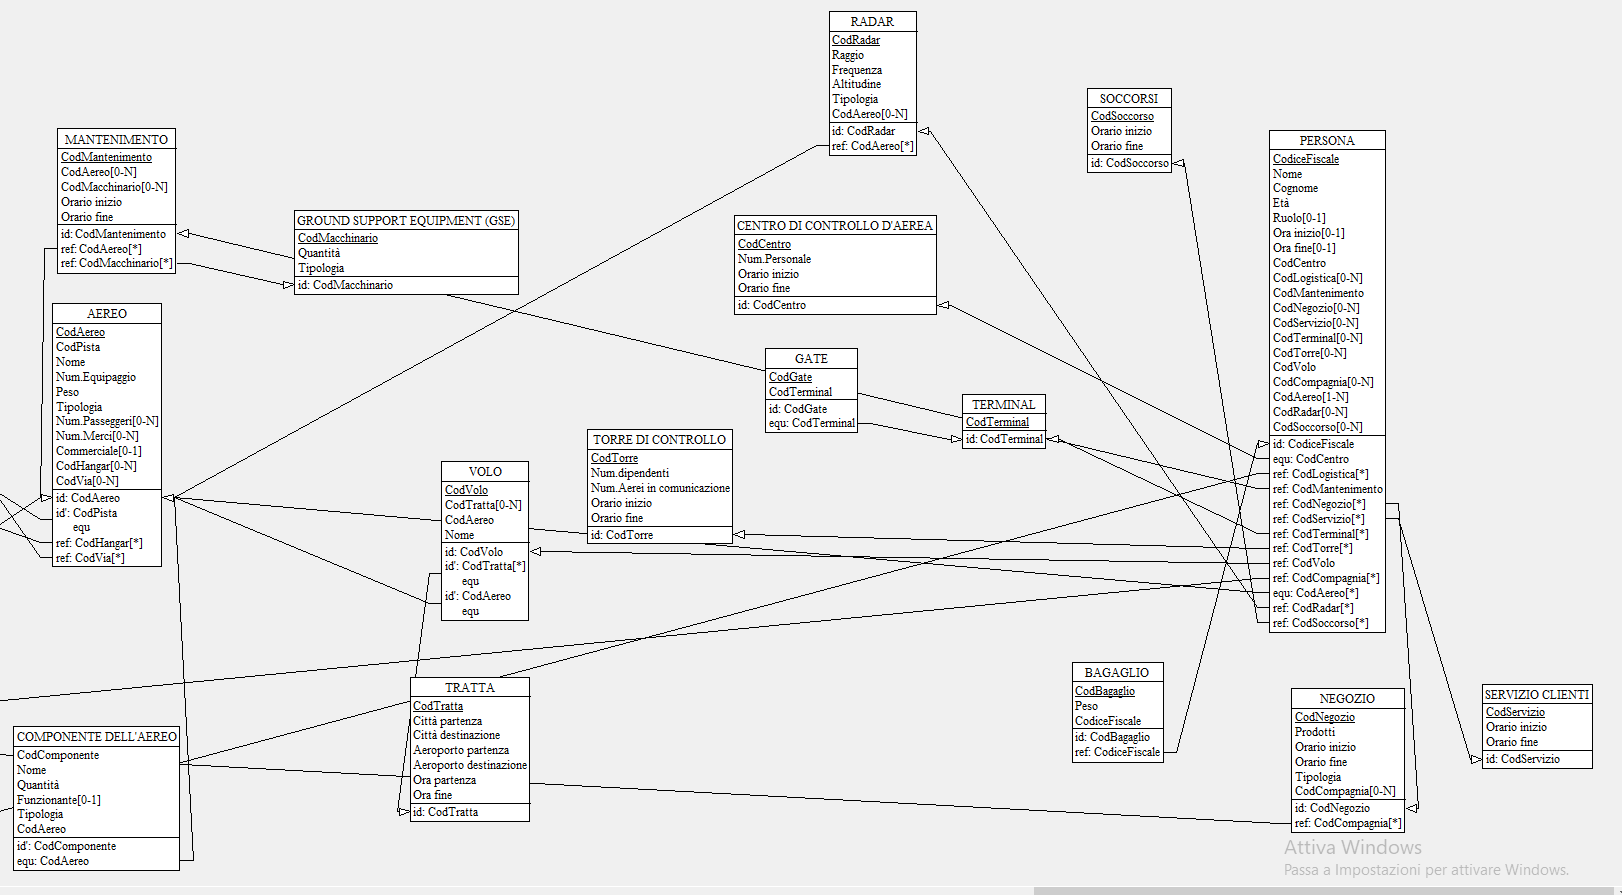
\includegraphics[width=1.2\textwidth]{./img/Schema_Logico/Schema_Logico1.png} %TODO: 1 o 1.1 o 1.2, con 1.2 perdiamo delle informazioni, ma si vedo meglio
	%\caption{}
	\label{fig:logico1}
\end{sidewaysfigure}

\begin{sidewaysfigure}[H]
	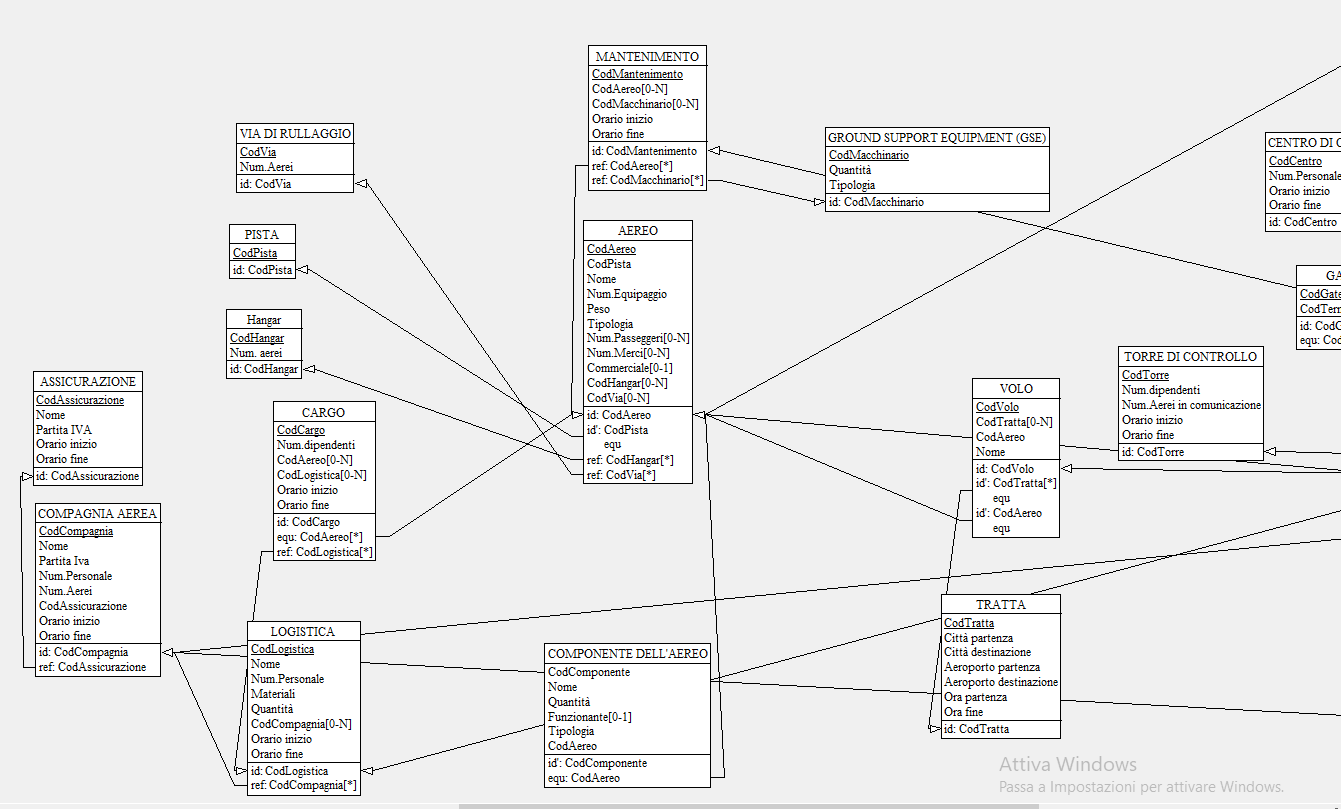
\includegraphics[width=1.2\textwidth]{./img/Schema_Logico/Schema_Logico2.png}
	%\caption{}
	\label{fig:logico2}
\end{sidewaysfigure}
\end{comment}

\begin{figure}[H] 
	\centering
	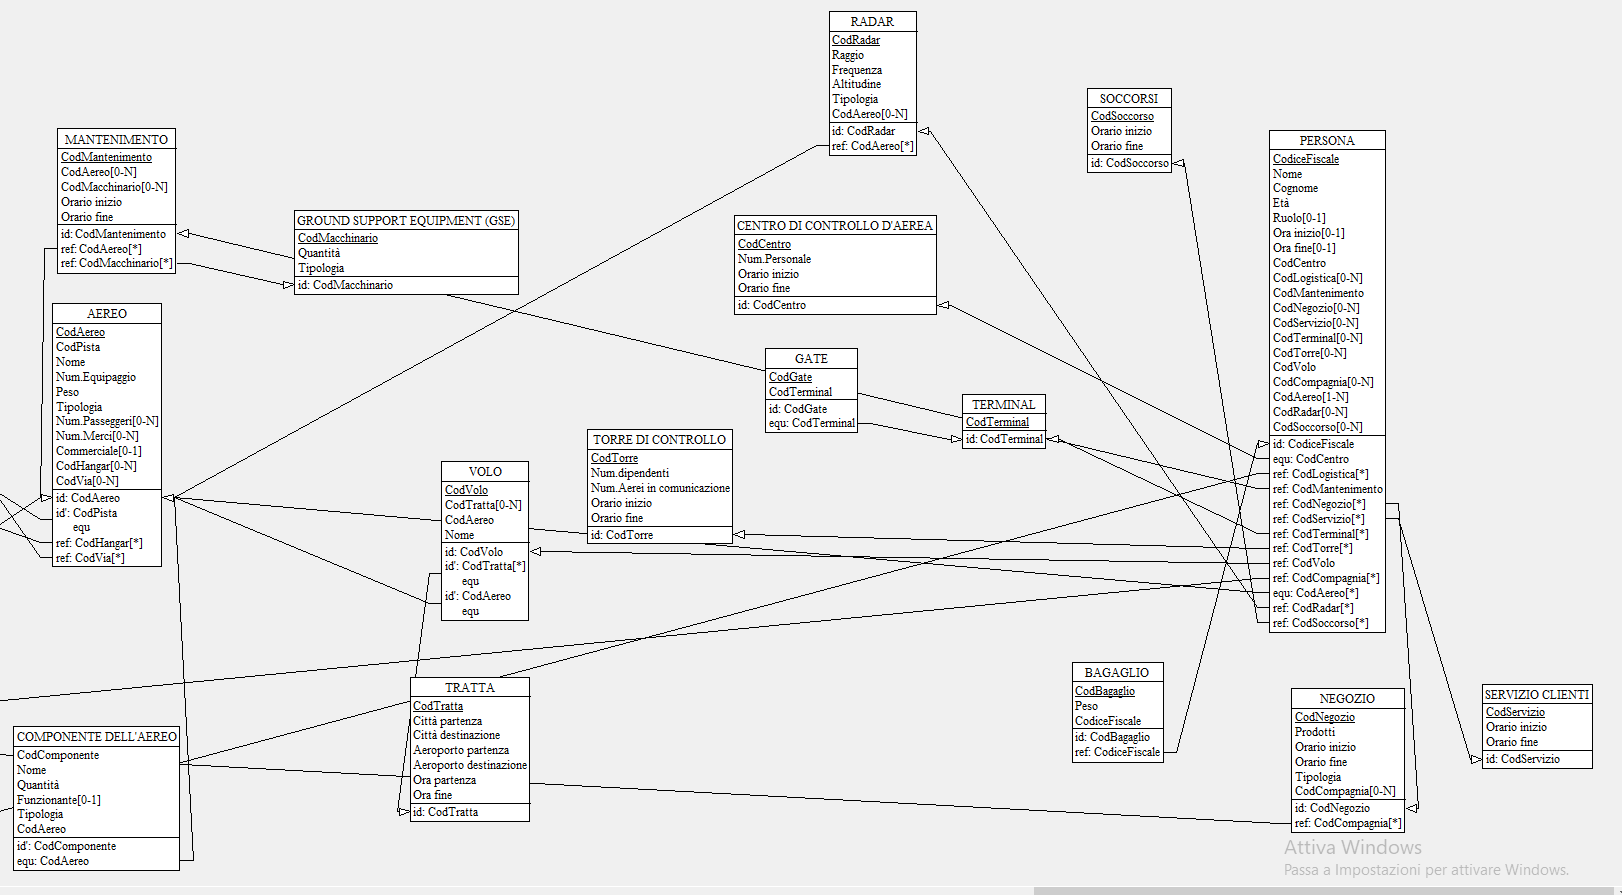
\includegraphics[width=1.2\linewidth, height=1.2\textheight, keepaspectratio]{./img/Schema_Logico/Schema_Logico1.png} 
	\caption{Schema concettuale Logico 1.}
	\label{fig:schema_logico1}
\end{figure}

\begin{figure}[H] 
	\centering
	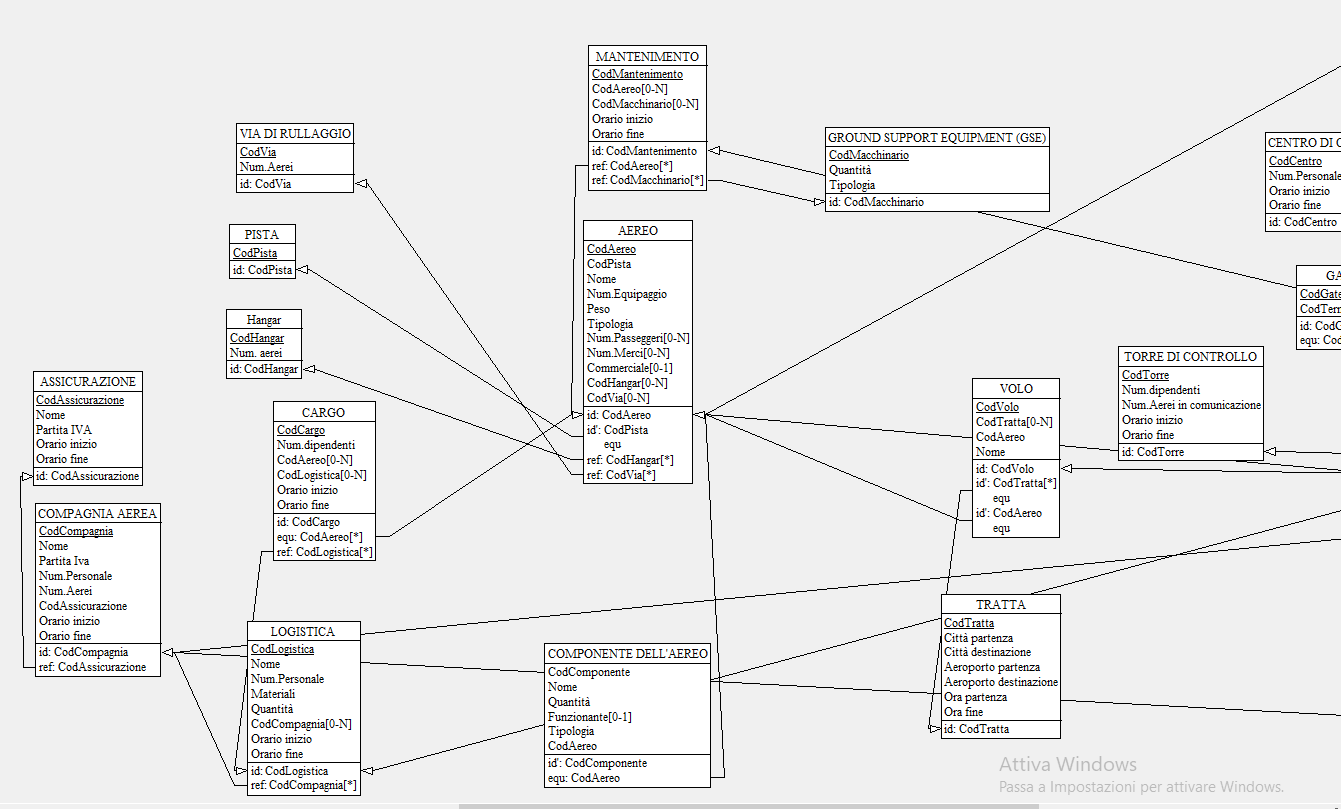
\includegraphics[width=1.2\linewidth, height=1.2\textheight, keepaspectratio]{./img/Schema_Logico/Schema_Logico2.png}
	\caption{Schema concettuale Logico 2.}
	\label{fig:schema_logico2}
\end{figure}

\restoregeometry

% --------------- TRASFORMAZIONE DELLE OPERAZIONI IN QUERY SQL -----------------

\newpage

% oppure riproposizione delle operazioni in query sql
\subsection{Trasformazione delle operazioni in query SQL}

% OP 1 | Registrare un nuovo passeggero

\textbf{\small OP 1 | Registrare un nuovo passeggero}

%\begin{comment}
	
\begin{lstlisting}[language=SQL]
INSERT INTO aeroporto.persona (CodiceFiscale, Nome, Cognome, Età, Ruolo,  CodVolo )
VALUES(?, ?, ?, ?, ?, ?); 
\end{lstlisting} 

%\end{comment}
% OP 2 | Numero totale di componenti non funzionanti in un aereo.

\textbf{\small OP 2 | Numero totale di componenti non funzionanti in un aereo}\\

\begin{lstlisting}[language=SQL]
SELECT COUNT(Funzionante) AS Num_Componenti_Non_Funzionanti
FROM aeroporto.aereo A JOIN aeroporto.componente_aereo CA ON A.CodAereo = CA.CodAereo
WHERE A.CodAereo = ?
AND CA.Funzionante = ?;
\end{lstlisting}

% OP 3 | Voli in partenza

\textbf{\small OP 3 | Voli in partenza}\\

\begin{lstlisting}[language=SQL]
SELECT volo.CodTratta, CodVolo, Nome, Città_partenza, Città_destinazione, Aeroporto_partenza, Aeroporto_destinazione, Ora_partenza, Ora_fine
FROM aeroporto.volo, aeroporto.tratta 
WHERE aeroporto.volo.CodTratta = aeroporto.tratta.CodTratta
AND aeroporto.tratta.Aeroporto_partenza = ?
AND Ora_Partenza = ?;
\end{lstlisting}

% OP 4 | Voli in arrivo

\textbf{\small OP 4 | Voli in arrivo}\\

\begin{lstlisting}[language=SQL]
SELECT volo.CodTratta, CodVolo, Nome, Città_partenza, Città_destinazione, Aeroporto_partenza, Aeroporto_destinazione, Ora_partenza, Ora_fine
FROM aeroporto.volo, aeroporto.tratta
WHERE aeroporto.volo.CodTratta = aeroporto.tratta.CodTratta
AND aeroporto.tratta.Aeroporto_destinazione = ?
AND Ora_fine = ?;	
\end{lstlisting}

% OP 5 | Manutenzione di un aereo

\textbf{\small OP 5 | Manutenzione di un aereo}\\

\begin{lstlisting}[language=SQL]
SELECT CodMantenimento, CodMacchinario, aeroporto.mantenimento.CodAereo
FROM aeroporto.mantenimento, aeroporto.aereo
WHERE aeroporto.mantenimento.CodAereo = aeroporto.aereo.CodAereo;	
\end{lstlisting}

% OP 6 | Comunicazioni tra controllori e membri dell'equipaggio di un aereo

\textbf{\small OP 6 | Comunicazioni tra controllori e membri dell'equipaggio di un aereo}\\

\begin{lstlisting}[language=SQL]
SELECT Num_Aerei_in_comunicazione
FROM aeroporto.torre_di_controllo
WHERE CodTorre = ?; 	
\end{lstlisting}

% OP 7 | Rifornimento di un aereo

\newpage %\pagebreak

\textbf{\small OP 7 | Rifornimento di un aereo}\\

\begin{lstlisting}[language=SQL]
SELECT *
FROM aeroporto.logistica, aeroporto.cargo
WHERE logistica.CodLogistica = cargo.CodLogistica
AND logistica.Materiali = ?;	
\end{lstlisting}

% OP 8 | Assunzione di nuovi addetti

\textbf{\small OP 8 | Assunzione di nuovi addetti}\\

\begin{lstlisting}[language=SQL]
INSERT INTO aeroporto.persona (CodiceFiscale, Nome, Cognome, Età, Ruolo, Ora_inizio, Ora_fine) VALUES (?, ?, ?, ?, ?, ?, ?);
\end{lstlisting}

% OP 9 | Controllare numero di radar presenti all'aeroporto

\textbf{\small OP 9 | Controllare numero di radar presenti all'aeroporto}\\

\begin{lstlisting}[language=SQL]
SELECT COUNT(CodRadar) AS Num_Radars
FROM aeroporto.radar;
\end{lstlisting}

% OP 10 | Aerei nella Via di Rullaggio

\textbf{\small OP 10 | Aerei nella Via di Rullaggio}\\

\begin{lstlisting}[language=SQL]
SELECT Num_Aerei
FROM aeroporto.via_di_rullaggio
WHERE CodVia = ?;	
\end{lstlisting}

% OP 11 | Acquirenti ai negozi

\textbf{\small OP 11 | Acquirenti ai negozi}\\

\begin{lstlisting}[language=SQL]
SELECT COUNT(P.CodiceFiscale) AS Num_Clienti
FROM aeroporto.negozio N JOIN aeroporto.persona P on P.CodNegozio = N.CodNegozio
WHERE P.CodNegozio = ?;
\end{lstlisting}

% OP 12 | Passeggeri che si recano al Terminal

\textbf{\small OP 12 | Persone che si recano al Terminal}\\

\begin{lstlisting}[language=SQL]
SELECT COUNT(P.CodiceFiscale) AS Persone_Al_Terminal
FROM aeroporto.terminal T JOIN aeroporto.persona P ON T.CodTerminal = P.CodTerminal
WHERE P.CodTerminal = ?;
\end{lstlisting}

% OP 13 | Nuovi membri dell'equipaggio assunti da una compagnia

\textbf{\small OP 13 | Nuovi membri dell'equipaggio assunti da una compagnia}\\

\begin{lstlisting}[language=SQL]
INSERT INTO aeroporto.persona ( CodiceFiscale, Nome, Cognome, Età, Ruolo, Ora_Inizio, Ora_fine, CodAereo )
VALUES ( ?, ?, ?, ?, ?, ?, ?, ? )	
\end{lstlisting}

% OP 14  | Inserimento di aerei stazionati negli Hangar

\textbf{\small OP 14 | Inserimento di aerei stazionati negli Hangar}\\

\begin{lstlisting}[language=SQL]
INSERT INTO aeroporto.aereo ( CodAereo, CodPista, Nome, Num_Equipaggio, Peso, Tipologia, CodHangar)
VALUES( ?, ?, ?, ?, ?, ?, ?);	
\end{lstlisting}

% OP 15 | Calcolare l'età media dei passeggeri

\textbf{\small OP 15 | Calcolare l'età media dei passeggeri}\\

\begin{lstlisting}[language=SQL]
SELECT AVG(Età) AS Media_Età
FROM aeroporto.persona
WHERE Ruolo = "Passeggero";	
\end{lstlisting}

% OP 16  | Ottenere il numero di aerei di una compagnia aerea

\pagebreak

\textbf{\small OP 16 | Ottenere il numero di aerei di una compagnia aerea}\\

\begin{lstlisting}[language=SQL]
SELECT Num_Aerei
FROM aeroporto.compagnia_aerea
WHERE CodCompagnia = ?;	
\end{lstlisting}

% OP 17  | Numero di controllori in una Torre di Controllo

\textbf{\small OP 17 | Numero di controllori in una Torre di Controllo}\\

\begin{lstlisting}[language=SQL]
SELECT Num_dipendenti
FROM aeroporto.torre_di_controllo
WHERE CodTorre = ?;	
\end{lstlisting}

% OP 18  | Numero di macchinari presenti nell'Aeroporto

\textbf{\small OP 18 | Numero di macchinari presenti nell'Aeroporto}\\

\begin{lstlisting}[language=SQL]
SELECT SUM(Quantità) AS Num_Totale_Macchinari
FROM aeroporto.ground_support_equipment;	
\end{lstlisting}

% OP 19  | Mostrare i controllori che erano in servizio dalle 08:00 alle 13:00

\textbf{\small OP 19 | Mostrare i controllori che erano in servizio dalle 08:00 alle 13:00}\\

\begin{lstlisting}[language=SQL]
SELECT CodiceFiscale, Nome, Cognome, Età, CodTorre, CodCentro, Ora_inizio, Ora_fine
FROM aeroporto.persona
WHERE Ruolo = "Controllore"
AND Ora_inizio >= CAST(? AS TIME)
AND Ora_fine <= CAST(? AS TIME)
GROUP BY Cognome;	
\end{lstlisting}

% OP 20  | Numero aerei commerciali di una compagnia aerea

\textbf{\small OP 20 | Numero aerei commerciali di una compagnia aerea}\\

\begin{lstlisting}[language=SQL]
SELECT COUNT(Commerciale) AS Num_Aerei_Commerciali
FROM aeroporto.aereo
WHERE Commerciale = ?;
\end{lstlisting}

% OP 21  | Quantità di merci trasportate in media da un aereo commerciale

\textbf{\small OP 21 | Quantità di merci trasportate in media da un aereo commerciale}\\

\begin{lstlisting}[language=SQL]
SELECT AVG(Num_Merci) AS Media_Merci_Trasportate
FROM aeroporto.aereo;	
\end{lstlisting}